\chapter{Automated Sentence Assignment to the Domain Experts}

%\atrcomments{contains the RANLP experiments}

\section{Introduction}

POS tagging and dependency parsing may not perform reasonably well for out-of-domain/ heterogeneous datasets. This means that a tagger/parser trained on a homogeneous dataset, e.g., Penn Treebank works reliably well on a similar dataset but fails to achieve similar results for heterogeneous datasets. In the previous chapter, I approached this problem by creating genre/domain experts using topic modeling: I use Latent Dirichlet Allocation (LDA)~\citep{Blei:2003:LDA:944919.944937,Blei:2012:PTM:2133806.2133826} for an unsupervised clustering of  sentences into topics. The assumption is that these topics correspond to genres. We observed that the topic modeler models the split into genres in a very similar way to the original split, with error rates around 2\%. I then train one expert per topic. I.e., I train the expert on all the training sentences that were assigned to the corresponding topic. 
%During testing, I assign test sentences to topics, which means that they are POS tagged and parsed by the corresponding expert.  I tested the approach on an artificial, heterogeneous corpus, consisting of a balanced mix of sentences from the WSJ portion of the Penn Treebank (financial news)~\citep{marcus:kim:ea:94} and from the GENIA corpus (biomedical abstracts)~\citep{tateisi:tsujii:04}. For POS tagging, there is a moderate increase in performance over a competitive baseline of training on the full training set, and a considerable increase for dependency parsing.
However, assigning test sentences to the relevant training topic experts is handled in the simplest possible way: I perform topic modeling on the combination of training and test data due to the non-parametric nature of the algorithm. Since topic modeling clusters the data but does not create a predictive model, we cannot assign sentences to topics after the initial clustering. 
This means that each time a new test sentence is encountered, the topic modeler would need to be rerun to consistently determine the appropriate genres across training and test sentences. In order to avoid retraining, I propose to use similarity estimation techniques to determine which genre the test sentence belongs to. In this setup, I only create the experts once with the training data, and then assign new sentences to genres in an asynchronous fashion. 
For a new test sentence, I evaluate the similarity of the test sentence to the sentences of a genre and then assign it to the expert with the highest similarity score. I investigate a range of different techniques, based on 1) words closely associated with a topic by the LDA, 2) $k$-nearest neighbors, or 3) perplexity models to estimate the similarity. 

%\atrcomments{needed?}The results indicate that for word based similarity metrics reach results very similar to the joint topic modeling approach, thus proving the feasibility of an asynchronous approach. In the case of unigram-based perplexity, parsing accuracy even surpasses the joint modeling approach.

The remainder of this chapter is structured as follows: \atrcomments{TBD}
 % The remainder of the paper is structured as follows: Section~\ref{problemstat} outlines our system architecture in greater detail, and section~\ref{relatedwork} discusses related work. In section~\ref{sim}, we describe the similarity methods, section~\ref{exptsetup} describes the setup for the experiments, and section~\ref{exptres} shows the results of our experiments.  In section~\ref{conc}, we draw conclusions and discuss future steps.
 
\section{Research Questions}

I demonstrated the usefulness of using POS tagging and parsing experts in the previous chapter. %However, assignment of sentences to experts is not automated. 
In this chapter, I address this issue by automatically assigning sentences to the corresponding experts. In other words, I primarily focus on the following:
\begin{enumerate} [label=\textbf{Question \arabic*:},align=left, leftmargin=!]

    \item \textbf{How do we assign sentences to domain/genre experts?}
    
    In this question, I focus on some of the methods used in estimating the similarity between documents. The idea is, given a cluster of sentences forming an expert, I estimate the similarity between these sentences and a test sentence. I then assign the sentence to the genre that it is most analogous to. I use techniques such as topic words from LDA, k-nearest neighbors and language model perplexity. Since I use the WSJ+GENIA mixed corpus (see section~\ref{sec:wsjgeniamixedcorpus}), I already have sentences tagged for domain/genre. This enables me to evaluate the performance of the methods in assigning sentences to genres. This also serves as an intrinsic evaluation. I.e., in this question, I judge the effectiveness of these techniques to classify a sentence to a genre expert.
    
    \item \textbf{How does POS tagging benefit from this asynchronous assignment?}
    
    In this question, I evaluate the advantage of using asynchronous assignment over retraining the topic modeler. I report on the overall accuracy of the part of speech tagger for asynchronous assignment against retraining. So, I use extrinsic evaluation. I.e., I evaluate the results end to end. This ascertains whether I get improvements on overall performance of the expert-based system when I implement these techniques to sort sentences to their corresponding expert.
    
    \item \textbf{How does dependency parsing benefit from this asynchronous assignment?}
    
    In the previous question, I asses the performance for POS tagger. In this question, I follow the same process for dependency parsing. I.e., I gauge the overall performance of the parser based on the Labeled Attachment Scores (LAS) and the Unlabeled Attachment Scores (UAS).
    
    \item \textbf{If there is an improvement overall, where does that stem from?}
    
    It is important to note the effect of correct genre assignment on overall performance of the POS tagger and dependency parser. In this question, I run experiments on the best settings to determine the effect of correct genre assignment on the end-to-end performance of the expert-based system. 



\end{enumerate}




\section{ System Overview}\label{problemstat}
\todo[inline]{Do I need to cite knn, dice coeff, ig/gain ratio,perplexity?}

\subsection{Overall Architecture}
\begin{figure*}[t]
    \centering
    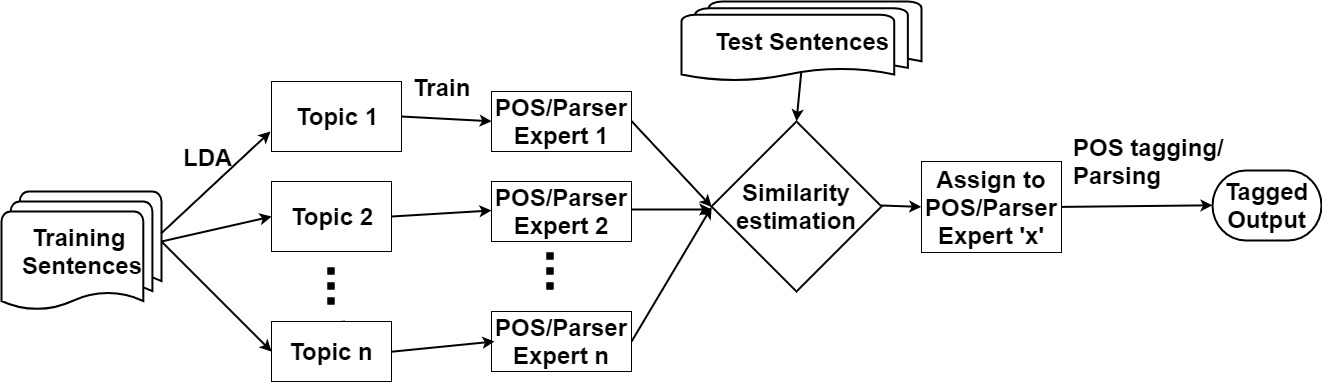
\includegraphics[width=\textwidth]{figures/approach-new.jpg}
 \caption{Overview of the architecture of the POS tagging and parsing experts.}\label{fig:architecture}   
 \end{figure*}


The training part of the process remains same as shown in figure~\ref{fig:architecture0} - LDA~\citep{Blei:2012:PTM:2133806.2133826,Blei:2003:LDA:944919.944937} is used to generate genres and train genre experts. In this chapter, I focus on the 2-topics case, which is the closest approximation for the mixed domain adaptation problem. Since in this case, we observed the best performance using hard clustering, I will use this as the base setting for similarity estimation experiments. 
I use 2 topics as prior, parallel to the 2 domains, and assign each training sentence via hard clustering to the genre for which LDA showed the highest probability.%\footnote{We have experimented with more topics for POS tagging and shown that we reach good results when using soft clustering rather than hard clustering \cite{mukherjee-kubler-scheutz:2016:W16-63}. The same holds true for experiments within the Penn Treebank, where we model WSJ internal topics, which are less distinct in their textual characteristics, but the experts still show an improvement over a full training baseline.}.  
I then test the different similarity metrics: I compute the similarity of a test sentence to the training sentences of the individual experts and then assign the sentence to the expert for tagging/parsing for which it has the highest similarity. I use techniques such as topic words from LDA, $k$-nearest neighbors \& language model perplexity for estimating similarity. Detailed description of these techniques are given below. I substantiate the use of these metrics as similarity estimation techniques in the next section.

\subsection{Similarity estimation Techniques}

\subsubsection{Topic words from LDA }
	
LDA does not only cluster sentences into genres, it also determines which words are highly correlated with each genre. Thus, we can utilize these words along with their probabilities for a specific genre. I sum over all genre words that we find in the sentence, weighted by their probability, and then assign the sentence to the topic that has the highest score. I explain it in details below:
%In the next section, I describe the process of using topic words as a similarity metric in detail.
%In this section, I explore whether we can define a metric from topic modeling that can be used for similarity estimation.

LDA provides a list of the words  which most closely associated with a topic and assigns a weight to each word.  So, the words that are highly correlated with each topic can be considered as good indicators for a sentence belonging to the genre represented by the topic. Additionally, I utilize the weights for each word assigned by LDA to determine a word's contribution to the similarity. For this experiment, I select the top 50/100/200 words from each topic. I.e., I assume that these words can be considered to be the most representative  words in their respective domain. Then, for each sentence, I check how many of those words occur in the current sentence and add up their weights. So for each test sentence, I compute the weights for each domain experts as follows: 

\begin{align}
    W_{t_j} = \sum_{i=1}^{N} w_{t_j}^{i}
\end{align}

$W_{t_j}$ is the overall weight for a test sentence for the $j^{th}$ topic; $w_{t_j}^{i}$ is the topic weight for the $i^{th}$ top word for the training topic expert; $N = 50/100/200$.

I then assign the sentence to the topic with the higher value. Since I only look at a small number of words, I have to consider the cases where a sentence does not contain any of the topic words. I resolve these cases by extending beyond the top  words and considering all the words in the training set for each genre. If there is a tie in values, we assign the sentence randomly to one of the experts. %The algorithm is given as below in~\ref{}
%\atrcomments{TBD: expand}
% \begin{algorithm}[!t]
% \caption{Topic words as similarity metric}
% \begin{algorithmic}[1]

% \end{algorithmic}
% \end{algorithm}

	
\subsubsection{ $k$-nearest neighbors} 
There exist a wide range of metrics to calculate similarity between two feature vectors. However, since I compare a sentence to a set of genre sentences, I decided to use memory-based classification using the  $k$-nearest neighbors to classify each test sentence into the relevant class (or genre, in our case). $k$-nearest neighbor is a supervised, non-parametric lazy learning algorithm. This has the advantage over a pure similarity metric that we have a principled way of handling the comparison to a set of sentences. Additionally, I do not consider the whole search space, as I would if I used a centroid.
	
 The typical steps for the algorithm is given as follows:

\begin{itemize}
    \item  The training data is stored in memory as feature vectors and associated class labels.
    \item The value of $k$ can be determined on a validation set based on the training errors for different $k$.
    \item For each datapoint in test, we do the following:
    \begin{itemize}
        \item We calculate the distance between the datapoint and each training data vector. Usually there are several metrics such as Euclidean distance, Cosine Similarity, etc.
        \item We sort these distances and consider the top $k$ values. 
        \item We choose the most frequent class from these and return it to be the predicted class for the test datapoint.
    \end{itemize}
\end{itemize}

TiMBL~\citep{daelemans1998timbl} enables us to implement variety of parameters to find the most optimum results. %Given below is the detailed description of the parameters which I used with $k$-nearest neighbors. 
I create a feature vector by using the top 50/100 words from each genre, as determined by LDA, and assigning the weights as values. The class label is the domain-membership, i.e., either WSJ or GENIA.

The classification parameters are determined by tuning these on a validation set. The settings are shown in table~\ref{tab:parameters}. It is based on the setting which had least training/validation errors. I explain these metrics in the next paragraphs.

\begin{table}[t]
\centering
\begin{tabular}{c|c|c|c}
\begin{tabular}[c]{@{}c@{}}Feature Vector\\  Size\end{tabular} & \begin{tabular}[c]{@{}c@{}}Number of\\ Nearest Neighbor\end{tabular} & Distance Metric & Feature Weighting \\ \hline
50 & 7 & Dice Coefficient & Gain Ratio \\
100 & 3 & Dice Coefficient & Gain Ratio \\ \hline
\end{tabular}
\caption{Classification parameters for $k$-nearest neighbors}
\label{tab:parameters}
\end{table}


\paragraph*{\textit{Dice Coefficient}}

Dice coefficient computes the similarity between two samples. In terms of set theory, this can be shown as:

\begin{equation} \label{eq:dc}
    DC(X,Y) ={\frac {2|X\cap Y|}{|X|+|Y|}}
\end{equation}

For language, dice coefficient can be used to calculate the number of common occurrences of character bigrams in the strings. Thus, given two strings $x$ and $y$, \ref{eq:dc} can be rewritten as:
\begin{equation}
    DC(x,y) = \frac{2n_{x \cap y}}{n_x + n_y}
\end{equation}

where $n_x$ is the number of character bigrams for string $x$ and $n_y$ is the number of character bigrams for string $y$.
Since we need to measure dissimilarity/distance rather than similarity, our metric is computed as below:
\begin{equation}
    d(x,y) = 1 - { \frac{2n_{x \cap y}}{n_x + n_y}}
\end{equation}

\paragraph*{\textit{Gain Ratio}}

In the previous paragraph, I discussed Dice Coefficient as the distance metric used in $k$-NN. However, it is a naive assumption that, all features are equally predictive of class labels. In other words, there are some features which are more informative than others. If we assume all features weigh same, we disregard this concept. Hence it is important to weigh features based on their predictive power. 

One of the widely used weighting scheme is Information Gain (IG). It measures how informative a feature is, to determine the class label. It relates to entropy which measures the amount of ``randomness" or uncertainty in a probability distribution. Entropy is represented as:
\begin{equation}
   H(Y) = -\sum_{y \in Y}  p(y)logp(y) 
\end{equation}
where $Y$ is a random variable. In this case, $Y$ can be considered as set of class labels such that $y \in Y$. 
Now, when we have the information on the value of the feature, we can compute a conditional entropy as below. 

% H(Y | X) = Si p(xi) H(Y | X=xi)
% H(C|v) = p(v) H(C|v) 
\begin{equation}
    H(Y|x) = \sum_{x \in X_n} p(x)H(Y|x)
\end{equation}

where $X_n$ is the value of the $n$-th feature.


Therefore, we can define information gain as difference between the overall entropy and the entropy conditional on the value of the feature. 

\begin{equation}
    IG(Y,x) = H(Y) - H(Y|x)
\end{equation}

While it is one of the commonly used metric, information gain tends to bias towards features with greater number of values i.e., the multi-valued features. Thus, a feature which is a good indicator of class label but contains lower number of values could potentially not given enough importance in information gain. To counter this effect, gain ratio is introduced, which normalizes information gain using a value referred to as split information (SI). This measures entropy on the value of the features. Thus SI is given as:
\begin{align}
    SI(n) = - \sum_{x \in X_n} p(x)logp(x)
\end{align}
Gain ratio can be represented as following:
\begin{align}
    Gain\ ratio = \frac{IG(Y,x)}{SI(n)}
\end{align}



%\item : Another obvious choice for determining the similarity of a sentence to a set of sentences is language modeling.  I calculate the perplexity of a test sentence with regard to set of sentences of an expert. I then assign a sentence to the expert for which it has the lowest perplexity. 
\subsubsection{Language Model Perplexity} 

As the third set of methods, I turn to language modeling and use perplexity as a measure to determine the similarity. I have two training experts, specializing in both domains in question. I calculate the perplexity of a test sentence to the experts. I then assign this test sentence to the expert which exhibits lower perplexity. I estimate unigram, bigram and trigram perplexity. I explain the concept in details below. I derive $n$-grams  of the training experts with additive smoothing using NLTK~\citep{loper2002nltk}, and compute the perplexity of the training experts to a test sentence

Language models assign probabilities to the sequence of words in a sentence~\citep{jurafsky2014speech}. It is essential to compute the most likely word that follows a sequence of words. N-gram is the simplest language model, which is a sequence of n words. We define a unigram, bigram and a trigram are sequences of one, two and three words respectively. If we consider a sentence to be a sequence of consequtive words,  $S = {w_1,w_2,...,w_n}$, the primary goal of a language model is to estimate the following:
\begin{align}
    P(S) = P(w_1,w_2,..w_n)
\end{align}
According to the chain rule of probability, we can calculate this as:
\begin{equation}
    \begin{aligned}
        P(w_1,w_2,..w_n) &= P(w_1)P(w_2|w_1)P(w3|w_1,w_2) ... P(w_n|w_1,..w_{n-1})&&\\
     &= \prod_i P(w_i|w_{1}^{i-1})&&
    \end{aligned}
\end{equation}

So, in order to find n-th word, we can simply estimate, $P(w_n|w_{n-1}, w_{n-2}, ... w_1)$. However, estimating conditional probabilities for sequences of any length is intractable and it is also nearly impossible to see all the probable sequences in the training data. Thus, it does not generalize well. Hence, we can make the Markov assumption, i.e., the future state depends on the current state only. In terms of language, this translates as:
\begin{align}
    P(w_1,w_2,..w_n) \approx \prod_i P(w_i|w_{i-k}..w_{i-1})
\end{align}

For a bigram model, we can make the following approximation:
\begin{align}
 P(w_i|w_1,w_2,..w_{i-1}) \approx P(w_i|w_{i-1})
\end{align}

We use maximum likely estimates (MLE) to calculate these probabilities. Hence,
\begin{align}
    P(w_i|w_{i-1}) = \frac{Count(w_{i-1}w_i)}{Count(w_{i-1})}
\end{align}

This means that, we calculate bigram probability of a word $w_n$, given the previous word $w_{n-1}$ by counting the number of times these words appear in conjunction in our corpus, normalized by the number of times $w_{n-1}$ appears in the corpus. 
Once we know these probabilities, it is trivial to estimate the most likely word that follows a sequence of words.  

There is an extrinsic evaluation method for language models, i.e., we use language model and then measure the end to end performance of a system. E.g., if we want to use language models for a machine translation system, we can judge the efficiency of using language model by simply evaluating the MT system. However, I discuss one of the widely used intrinsic evaluation method, perplexity. Perplexity is a function of probability of a sentence - it computes the inverse probability for an unseen test set, normalized by the number of words~\citep{jurafsky2014speech}. Hence, lower the perplexity, higher the probability, which implies that the model generalizes well.


\begin{equation}
    \begin{aligned}
    Perplexity(S) & = P(w_1,w_2,w_3, ... , w_n)^{-\frac{1}{n}} \\
    & = \sqrt[n]{\frac{1}{P(w_1,w_2,w_3, ... , w_n)}} \\
    & = \sqrt[n]{\prod_{i=1}^{n}\frac{1}{P(w_i|w_1, .. w_{i-1})}} \\
    \end{aligned}
\end{equation}
Thus, for bigrams, we can compute perplexity as:

\begin{equation}
    Perplexity(S) = \sqrt[n]{\prod_{i=1}^{n}\frac{1}{P(w_i|w_{i-1})}}
\end{equation}
    
    
\paragraph*{Smoothing}
Unknown or out of vocabulary (OOV) words are a major problem language model performance. Often a test set has words that never appeared in the training set. Thus the performance might suffer if we assign zero probability to these cases. The idea of smoothing is to ``reallocate" probability mass from seen $n$-grams to unseen ones. There are several smoothing methods. However, since I use additive smoothing, I discuss the methods as below:

\begin{itemize}
    \item Laplace smoothing: Adds one to the counts of $n$-grams before estimating the probabilities. This is the simplest smoothing technique.
    \item Add-k smoothing: Instead of adding one, we add a value $k$ to the counts. The value of $k$ can be determined on a validation set. 
\end{itemize}




% \subsection{Corpus}
% \todo[inline]{separate chapter?}

% I create a corpus manually by combining equal parts of Wall Street Journal(WSJ)~~\citep{marcus:kim:ea:94} section of the Penn Treebank and the GENIA corpus~\citep{tateisi:tsujii:04}. WSJ consists of newspaper reports while GENIA consists of biomedical abstracts from Medline. The corpus is balanced, it has equal representation from both the genres/domains. This artificially balanced corpus provides a perfect setting to run experiments to know which genre a sentence belongs to. 


% For the WSJ corpus, I use the POS annotation and syntactic annotations  from the treebank. The GENIA Corpus is annotated on different linguistic levels, including POS tags, syntax, coreference, and events, among others. I use GENIA 1.0 trees~\cite{Ohta:2002:GCA:1289189.1289260} created in the Penn Treebank format\footnote{http://nlp.stanford.edu/~mcclosky/biomedical.html}. Both treebanks are converted to dependencies using pennconverter~\cite{johansson2007a}.

% Following the data split in the previous chapter, I create a balanced dataset comprising 17~181 sentences from each corpus for the training set and 850 sentences for the test set. Since GENIA is rather small and since there is no standard data split for GENIA, I decided to extract the last 850 sentences for the test set, and the 850 sentences before that for the validation set. The remaining 17~181 sentences are used for training. For WSJ, I chose the same number of sentences for the training, validation,  and test set, the training sentences are selected randomly from sections 02-21 and the validation and test sentences from section 22 and 23 respectively.



\subsection{Baselines}

In the previous chapter, I have used two baseline cases: The first baseline considers the entire training set and does not employ any topic modeling. Since the topic experts have access to only a fraction of the data, a second and more comparable baseline consists of  randomly distributing  training and test sentences into sets that correspond in size to the genres. I use these baselines and add a third, which is more relevant to our current setting. In this case, I use the experts trained on the genres but then randomly assign test sentences to the experts. This allows me to gauge how important a correct assignment to the corresponding expert is. 


% \subsection{Similarity Estimation}

% For the $k$-nearest neighbor estimation, I use the Tilburg Memory-Based Learner (TiMBL) \citep{daelemans1998timbl}. For the perplexity models, I derive $n$-grams  of the training experts with additive smoothing using NLTK~\citep{loper2002nltk}, and compute the perplexity of the training experts to a test sentence~\footnote{For Topic Modeling, POS tagging \& Dependency Parsing, I use MALLET, TnT \& MATE respectively, as done in the previous chapters.}. 

\subsection{Evaluation}

The evaluation is two-fold - intrinsic \& extrinsic. As a part of intrinsic evaluation, I compute the accuracy of assigning sentences to its appropriate genre. For extrinsic or end-to-end evaluation, I use the script \texttt{tnt-diff} that is part of TnT to evaluate the POS tagging results  and the CoNLL shared task evaluation script\footnote{http://ilk.uvt.nl/conll/software/eval.pl} for evaluating the parsing results.


\section{Experimental Results} \label{exptres}

\subsection*{Question 1: How do we assign sentences to domain/genre experts?}

\begin{table*}[t!]
\centering
\begin{tabular}{l|l|r|}
Similarity metric & Setting & Accuracy \\ \hline
joint LDA & & 98.94 \\ \hline
topic words & 50 & 97.59 \\ 
 & 100 & 97.53 \\ 
 & 200 & 97.35 \\ \hline
perplexity & unigrams & \textbf{99.76} \\ 
 & bigrams & 84.71 \\  
 & trigrams & 81.53 \\ \hline
$k$-NN & 50 & 90.59 \\ 
 & 100 & 91.18 \\ \hline
\end{tabular}
\caption{Accuracy of genre assignment for different similarity metrics.}
\label{tab:acc:class:simmetr}
\end{table*}

I first investigate how well the different similarity metrics can assign the test sentences to the correct genre. I.e., I calculate accuracy in terms of whether a GENIA sentence is assigned to the GENIA genre, and a WSJ sentence to the WSJ genre.
Table~\ref{tab:acc:class:simmetr} shows the results of classification accuracy of using different similarity estimation techniques. The reference here is the joint LDA for training and test data, with an accuracy of 98.94\%. 
 
Perplexity based on unigrams reaches the highest accuracy, reaching an accuracy of 99.76\%, thus surpassing the joint LDA. Surprisingly, using bi- or trigrams instead decreases accuracy by 15-20 points absolute. I assume that this is due to data sparsity since the language model is trained on a relatively small dataset. The second highest accuracy is reached by the methods based on topic words. Here, the number of words considered does not seem to make a significant difference. The $k$-NN approach performs at around 91\%. These results indicate that using single words without context (i.e., the context in bi- and trigrams) provides the most reliable information. The language model has an additional advantage, potentially because it can smooth over unseen words.
  



  
\subsection*{Question 2: How does POS tagging benefit from this asynchronous assignment?}

\begin{table*}[!t]
\centering
\begin{tabular}{l|l|r|}
Setting & Similarity metric & Accuracy \\ \hline
full training &  & 96.69 \\ 
random split & & 96.41 \\ 
topic experts + random test &  & 91.36 \\ \hline
joint LDA &   & 96.95 \\ \hline
topic words & 50 & 96.80 \\ 
 & 100 & 96.81 \\ 
 & 200 & 96.81 \\ \hline
perplexity & unigrams & \textbf{96.92} \\ 
 & bigrams & 95.64 \\
 & trigrams & 95.22 \\ \hline
$k$-NN & 50 & 96.05 \\  
 & 100 & 96.09 \\ \hline
\end{tabular}

\caption{Results for the POS tagging experiments.}
\label{tab:overallresultspostag}
\end{table*}

Table~\ref{tab:overallresultspostag} shows the accuracies of the POS tagging experiments for different similarity metrics. We can see that assigning the test sentences randomly to genres has a detrimental effect, and reaches an accuracy of 91.36\%, which is more than 5 points absolute lower than the random split baseline. This difference shows how important it is that sentences are assigned to the correct genre.
 
Perplexity based on unigrams and the method using topic words reach comparable accuracies to the original topic expert results based on the joint LDA clustering. These results follow the same trends as the genre assignment accuracies, but the differences between the methods are smaller. The perplexity setting using unigrams does not only surpass the joint LDA scores but also all the baselines: by nearly 0.3 percent points for the full training set, by 0.5 percent points  for the random split, and by 5 percent points  for the random test assignment.





\subsection*{Question 3: How does dependency parsing benefit from this asynchronous assignment?}

  \begin{table*}[t!]
\centering
\begin{tabular}{l|l|rr|}
Setting &Similarity metric & LAS &UAS \\ \hline
full training & & 88.67 & 91.71 \\ 
random split &  & 87.84 & 90.86 \\ 
topic experts + random test &  & 82.17 & 88.13 \\ \hline
joint LDA & -& 90.51 & 92.14 \\ \hline
topic words & 50 & 90.30 & 92.07 \\
 & 100 & 90.30 & 92.07 \\
 & 200 & 90.30 & 92.07 \\ \hline
perplexity & unigrams & \textbf{90.54} & \textbf{92.16} \\
 & bigrams & 88.33 & 91.13 \\
 & trigrams & 87.50 & 90.68 \\ \hline
$k$-NN  &50 & 89.45 & 91.82 \\
 & 100 & 89.52 & 91.84 \\ \hline
\end{tabular}
\caption{Attachment scores for the dependency parsing experiments.}
\label{tab:overallresultsdep}
\end{table*}

Table~\ref{tab:overallresultsdep} shows labeled and unlabeled attachment scores of the dependency parses. These results mirror the trends in the POS tagging experiments: Randomly assigning sentences to genres results in the lowest LAS score of 82.17\%, and using perplexity based on unigrams reaches the highest LAS of 90.54\%. This LAS is considerably higher than the full training baseline of 88.67\%. Note that the differences between the accuracies based on different similarity metrics are considerably more pronounced than in the POS tagging experiments. This mirrors the trend that we have previously seen for the joint LDA assignment. It is also interesting to see that the results for all the topic word settings are the same. This is due to 5 sentences that did not contain any of the topic words and thus had to be randomly assigned to one genre. 


\subsection*{Question 4: If there is an improvement overall, where does that stem from?}

I now have a closer look at the two best settings, i.e., the perplexity experiment using unigrams and 50 topic words: I separate the sentences that were assigned to the wrong genre from the correctly assigned ones and evaluate them separately. For the unigram setting, 4 sentences were assigned to the wrong genre, for the 50 topic words, 41 sentences. The results are shown in Table~\ref{tab:comp}.  These results show that the sentences that were assigned to the wrong genre receive POS and dependency analyses with significantly lower accuracies, the difference to the correct ones ranging between 5 points absolute for POS tagging and 10-14 points for parsing. This corroborates my findings that the correct assignment to a genre is of utmost importance, which also corroborates my conclusion that the genre experts model genre-specific information. If they did not, mis-assigning sentences would not have any impact.

\begin{table*}[t]
\centering
\begin{tabular}{ll|rrr|}
 & Setting & Correct genre & Incorrect genre  & Overall \\ \hline
POS tagging (acc.) & unigram & 96.92 &  91.84 & 96.92\\
&  topic words 50 & 98.23 & 88.59 & 96.80\\
parsing (LAS) & unigram& 90.54& 85.72 & 90.54  \\
& topic words 50 & 90.55 & 76.19 & 90.30\\ \hline
\end{tabular}
\caption{Results for POS tagging and dependency parsing when we separate incorrectly assigned sentences from correct ones.}
\label{tab:comp}
\end{table*}

\section{Summary} \label{conc}

Using topic modeling to create experts can be very beneficial, but this approach is only viable if we can assign new sentences asynchronously to genres without having to retrain the LDA to determine genres that include the new sentences. I have investigated similarity based methods for assigning the new sentences to genres.
More specifically, I have  investigated the following methods:  1) using topic words that LDA associates with a genre, 2) $k$-nearest neighbor models, and 3) perplexity in language models. A baseline that assigns test sentences randomly to genres performs poorly, thus showing that the correct assignment to genres is indispensable.

The results show that the perplexity model  based on unigrams surpasses the accuracy of a joint LDA model that assigns the sentences synchronously.  For POS tagging, the  accuracy of the unigram perplexity model is very close to that of the joint LDA.  For parsing, the unigram perplexity model outperforms the joint LDA model.  Using the 50 topic words to assign sentences to their genre reaches accuracies close to the best performing model. This shows that word-based methods are more robust in comparison to bigram and trigram methods, which should be able to profit from more context but also face data sparsity issues.

\atrcomments{Not sure if this is needed}
As a part of future work, I plan to investigate models with a more dynamic mix of genres during the POS tagging and parsing process. I.e. rather than creating independent experts, I will investigate methods to create a POS tagger and parser that have access to expert views during each decision about the next POS tag or parsing step. I will also investigate whether I can integrate gold POS tags or dependency information into the topic modeling process, so that the topic modeler has access not only to the specialized lexical information but also to the linguistic information that it is ultimately tasked to distinguish. 
